%By Douglas Bish
%The text is licensed under the
%\href{http://creativecommons.org/licenses/by-sa/4.0/}{Creative Commons
%Attribution-ShareAlike 4.0 International License}.
%
%This file has been modified by Robert Hildebrand 2020.  
%CC BY SA 4.0 licence still applies.


We start with some preliminaries, and then discuss the simplex algorithm, assuming an initial basic feasible solution, including tableau formulas.  Next two extensions to the algorithm, for finding an initial basic feasible solution, are discussed. We then explore a useful algorithm for solving certain LPs that have``too many" columns.



Consider an LP $\text{max} \{\mathbf{cx}: \mathbf{Ax} = \mathbf{b}, \mathbf{x} \ge \mathbf{0} \}$ in standard form, where:  

\begin{itemize}
\item $\mathbf{A}$ is an $m \times n$ matrix of rank $m$ and $n \ge m$; $\mathbf{A}$ consists of $n$ column vectors, $\mathbf{a_1}, \mathbf{a_2}, \mathbf{a_3}, \cdots, \mathbf{a_n}$.
\item $\mathbf{c}$ and $\mathbf{x}$ are $n$-vectors.
\item $\mathbf{b}$ is an $m$-vector with non-negative elements.
\end{itemize}

We can partition the problem as $\mathbf{x}= [\mathbf{x_B}, \mathbf{x_N}]$, $\mathbf{A} = [\mathbf{B}, \mathbf{N}]$, $\mathbf{c}= [\mathbf{c_B}, \mathbf{c_N}]$, where:  

\begin{itemize}
\item $\mathbf{x_B}$ is the vector of basic variables
\item $\mathbf{B}$ is the {\it basis matrix}, a nonsingular (i.e., it consists of $m$ linearly dependent columns of $\mathbf{A}$) $m \times m$ matrix.
\item $\mathbf{c_B}$ is the vector of cost coefficients for the basic variables.
\item $\mathbf{x_N}$ is the vector of nonbasic variables
\item $\mathbf{N}$ is the {\it nonbasic matrix}, a $m \times n-m$ matrix.
\item $\mathbf{c_N}$ is the vector of cost coefficients for the basic variables.
\end{itemize}

The LP can then be written as:  
$$\text{max} \{\mathbf{c_Bx_B} + \mathbf{c_Nx_N}: \mathbf{Bx_B} + \mathbf{Nx_N} = \mathbf{b}, \mathbf{x_B, x_N} \ge 0\}.$$
For the feasible region, we can write the system of equations as follows: \\
$$\mathbf{B} \mathbf{x_B} + \mathbf{N} \mathbf{x_N} = \mathbf{b}.$$ 
$$\mathbf{B} \mathbf{x_B}  = \mathbf{b}-  \mathbf{N} \mathbf{x_N}.$$ 
Premultiplying by $\mathbf{B^{-1}}$ yields:  
$$\mathbf{x_B} = \mathbf{B^{-1}}\mathbf{b} - \mathbf{B^{-1}} \mathbf{N} \mathbf{x_N}.$$ 

By setting $\mathbf{x_N} = \mathbf{0}$ and solving we (potentially) find a {\it basic feasible solution} to the system, which corresponds to an extreme point of the feasible region. Remember that the nonbasic variables $\mathbf{x_N} = \mathbf{0}$ represent the defining hyperplanes for a solution. \\

For any set of $m$ variables, the result can be:

\begin{enumerate}
\item a basic feasible solution, $\mathbf{x_B} \ge \mathbf{0}$.
\item a basic infeasible solution, some $x \in \mathbf{x_B} \le 0$.
\item a set of linearly dependent columns that does not span the $m$-space.
\end{enumerate}

For this system there are possibly $n$ choose $m$ ${n \choose m}$ basic solutions, that is, the number of basic feasible solutions is bounded by $n!/m!(n-m)!$ from above.  \\

\subsubsection{The Simplex Algorithm}

It is common practice to put an LP into a tableau.  To do so, we first modify the objective function by bringing all the variables to the left-hand side, yielding the following tableau of LP data: 
\begin{center} \begin{tabular} {l|c|c|c|} \cline{2-4}
max                    					& $z$	        		  & $x_i$	               &  $rhs$  \\ \cline{2-4}
Row 0 ($z$)         		& 1	            		  & $-c_i$ 			  & $0$	    \\ \cline{2-4}
Rows 1-$m$                & $\mathbf{0}$ & $\mathbf{a_i}$ & $\mathbf{b}$  \\ \cline{2-4}
\end{tabular} \end{center}

We are interested in tableaus that represent basic solutions, which have a special form; the columns of coefficients for the basis to form an identity matrix, which we can obtain using elementary row operations. \\

\bigskip Consider the following LP:  
\begin{align*}
\mbox{Max~~} & z = 2x_1 + x_2  \\\
\mbox{s.t.~~} & x_1 - x_2 +x_3 =  2  \\
& x_1 + x_2 +x_4  = 3 \\
& x_1, x_2, x_3 , x_4  \ge 0,
\end{align*}
where $m$=2, $n$=4, $\mathbf{A}$=$\left[ \begin{array}{rrrr} 1 & -1 & 1 & 0 \\  1 &  1 &  0 & 1 \\ \end{array} \right],$ \\
$\mathbf{a_1}$=$ \left[ \begin{array}{c} 1  \\ 1  \\ \end{array} \right],$
$\mathbf{a_2}$=$\left[ \begin{array}{c} - 1  \\ 1  \\ \end{array} \right],$
$\mathbf{a_3}$=$\left[ \begin{array}{c} 1  \\ 0  \\ \end{array} \right],$
$\mathbf{a_4}$=$\left[ \begin{array}{c} 0  \\ 1  \\ \end{array} \right],$ \\
$\mathbf{c}$=$\left[ \begin{array}{rrrr} 2  & 1  & 0 & 0  \\ \end{array} \right],$ \\
$\mathbf{x}$=$\left[ \begin{array}{rrrr} x_1  & x_2  & x_3 & x_4  \\ \end{array} \right]^T,$ (T for transpose, $\mathbf{x}$ is a column vector), \\
and $\mathbf{b}$=$ \left[ \begin{array}{c} 2 \\ 3  \\ \end{array} \right].$\\

The tableau and graph for this LP follow:

\begin{minipage}[t][][b]{.50\linewidth} \vspace{2mm}
\begin{center} \begin{tabular} {l|c||c|c|c|c|c|}  \cline{2-7}
max & $z$	& $x_1$ & $x_2$  & $x_3$	& $x_4$	& $rhs$ \\ \cline{2-7}
($z$)	    & 1		& -2        &  -1        &	 0 	    &	  0		&   0    \\ \cline{2-7}
($x_3$)			& 0		&	 1        &     -1     &	 1 			&	  0 		&	  2   \\
($x_4$)			& 0		&	  1       &	    1    &	 0 		&	  1 		&	   3   \\ \cline{2-7}
\end{tabular} \end{center}
\end{minipage}%
\begin{minipage}[t][][b]{.50\linewidth}
\begin{center}  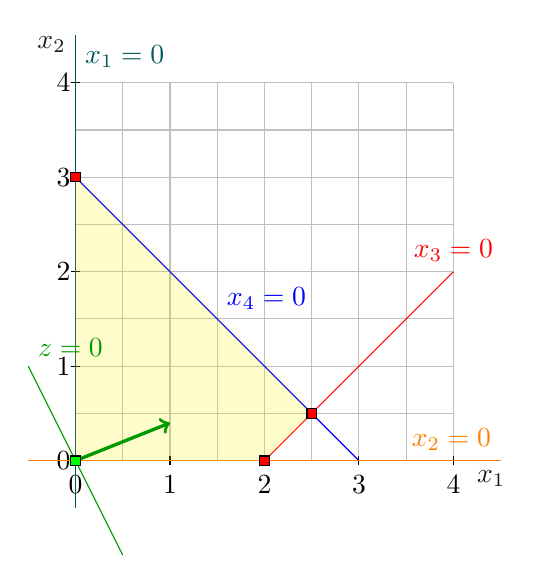
\begin{tikzpicture} [scale=1.2]
\draw[gray!50, thin, step=.5] (0,0) grid (4,4);
\draw[opacity=0.9] (0,0) -- (4.4,0) node[below] {$x_1$};
\draw[opacity=0.9] (0,0) -- (0,4.4) node[left] {$x_2$};

\foreach \x in {0,...,4} \draw (\x,0.05) -- (\x,-0.05) node[below] {\x};
\foreach \y in {0,...,4} \draw (-0.05,\y) -- (0.05,\y) node[left] {\y};

\draw [red](2, 0) --  (4, 2) node[above] {$x_3= 0$};
\draw [blue] (0,3)  -- node[above right] {$x_4=0$} (3,0) ;
\draw [teal!70!black](0,-.5) --  (0,4.5) node[below right] {$x_1=0$}; 
\draw [orange](-.5,0) --  (4.5,0) node[above left] {$x_2=0$}; 

\fill[yellow,opacity=0.2] (0,0) -- (2,0) -- (2.5,0.5) -- (0,3) -- cycle;

\draw [green!60!black] (-0.5, 1)  node[above right] {$z=0$} --  (0.5, -1)  ; % o.f.
\draw [green!60!black, very thick,->](0,0) -- (0+1, 0+2/5); % gradient

\filldraw[fill=green] (-0.05,-0.05) rectangle (0.05,0.05);
\filldraw[fill=red] (2.45,0.45) rectangle (2.55,0.55);
\filldraw[fill=red] (1.95,-0.05) rectangle (2.05,0.05);
\filldraw[fill=red] (-0.05,2.95) rectangle (0.05,3.05);    
\end{tikzpicture} \end{center} 
\end{minipage}

Luckily, this tableau already represents a basis, which has basic variables $\mathbf{x_B}=[x_3~x_4]^T$ (we can consider $z$ as a basic variable of sorts to complete the identity matrix).  Thus for this tableau we have $\mathbf{x_N}=[x_1~ x_2]^T$ ,
$\mathbf{B}$=$\left[ \begin{array}{rr} 1 & 0  \\  0 &  1 \\ \end{array} \right]$, 
$\mathbf{N}$=$\left[ \begin{array}{rr} 1 &-1  \\  1 &  1  \\ \end{array} \right]$.  This basic solution represents an extreme point if we set the nonbasic variables to zero, as we see in the graph of the LP in the nonbasic variable space. \\   

Here the basic variable values are $x_3 = 2$ and $x_4=3$, and $z = 0$. \\

The simplex algorithm (mostly), tableau version:
\begin{enumerate}
\item Put the LP into a standard form tableau, find a set of basic variables that form a feasible basis, and  modify the tableau to represent the basis using elementary row operations, we want the coefficients of the basic variables to form an identity matrix. 
\item Check optimality, for a maximization (minimization), if the Row~0 coefficients for the nonbasic variables are all nonnegative (nonpositive) then the basis is optimal. 
\item If the basis is not optimal, then find an adjacent basis that improves the solution. This will involve swapping one of the basic variables with a nonbasic variable to form a new basis. 
\item Select a nonbasic entering variable using Dantzig’s rule, specifically, for a maximization (minimization) problem pick the nonbasic variable with the smallest negative (largest positive) reduced cost. 
\item Select a variable to leave the basis.  Conceptually, as we increase the entering variable's value from zero, the values of the basis variables should change, the basic variable that goes to zero first is the leaving variable. To find the leaving variable, use the  ratio test.  For each row 1-$m$ having a positive coefficient in the entering variable column, divide the $rhs$ by the entering variable's (positive) coefficient. The basic variable corresponding to row with the smallest ratio is the leaving variable.  
\item Put the  tableau into the proper form for the new basis using elementary row operations and go to Step~2.
\end{enumerate}

\bigskip Consider the following example:

\begin{minipage}[t][][b]{.50\linewidth} \vspace{2mm}
\begin{center} \begin{tabular} {l|c||c|c|c|c|c|}  \cline{2-7}
max & $z$	& $x_1$ & $x_2$  & $x_3$	& $x_4$	& $rhs$ \\ \cline{2-7}
($z$)	    & 1		& -2        &  -1        &	 0 	    &	  0		&   0    \\ \cline{2-7}
($x_3$)			& 0		&	 1        &     -1     &	 1 			&	  0 		&	  2   \\
($x_4$)			& 0		&	  1       &	    1    &	 0 		&	  1 		&	   3   \\ \cline{2-7}
\end{tabular} \end{center}
\end{minipage}%
\begin{minipage}[t][][b]{.50\linewidth}
\begin{center}  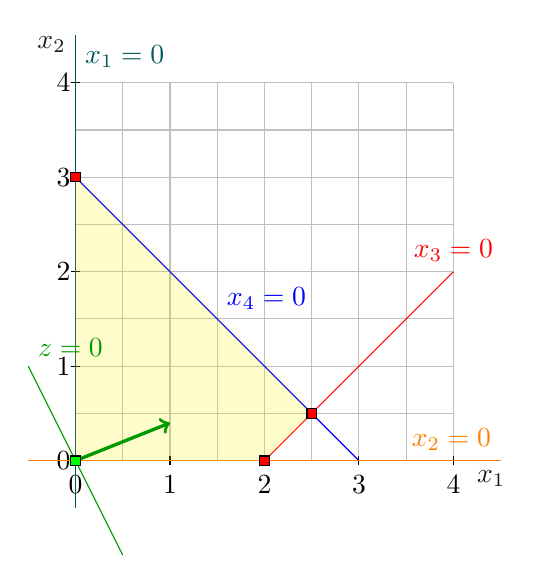
\begin{tikzpicture} [scale=1.2]
\draw[gray!50, thin, step=.5] (0,0) grid (4,4);
\draw[opacity=0.9] (0,0) -- (4.4,0) node[below] {$x_1$};
\draw[opacity=0.9] (0,0) -- (0,4.4) node[left] {$x_2$};

\foreach \x in {0,...,4} \draw (\x,0.05) -- (\x,-0.05) node[below] {\x};
\foreach \y in {0,...,4} \draw (-0.05,\y) -- (0.05,\y) node[left] {\y};

\draw [red](2, 0) --  (4, 2) node[above] {$x_3= 0$};
\draw [blue] (0,3)  -- node[above right] {$x_4=0$} (3,0) ;
\draw [teal!70!black](0,-.5) --  (0,4.5) node[below right] {$x_1=0$}; 
\draw [orange](-.5,0) --  (4.5,0) node[above left] {$x_2=0$}; 

\fill[yellow,opacity=0.2] (0,0) -- (2,0) -- (2.5,0.5) -- (0,3) -- cycle;

\draw [green!60!black] (-0.5, 1)  node[above right] {$z=0$} --  (0.5, -1)  ; % o.f.
\draw [green!60!black, very thick,->](0,0) -- (0+1, 0+2/5); % gradient

\filldraw[fill=green] (-0.05,-0.05) rectangle (0.05,0.05);
\filldraw[fill=red] (2.45,0.45) rectangle (2.55,0.55);
\filldraw[fill=red] (1.95,-0.05) rectangle (2.05,0.05);
\filldraw[fill=red] (-0.05,2.95) rectangle (0.05,3.05);    
\end{tikzpicture} \end{center} 
\end{minipage}

From the graph and tableau we can see that we are at the extreme point (0,0) and if we increase $x_1$ by one unit, the objective function ($z$-value) increases by 2, thus improving the solution.  We can increase $x_1$ by 2 and still remain in the feasible region, moving to extreme point (2,0).  Likewise, if we increase $x_2$ by one unit the objective function increases by 1, and we can increase $x_2$ by three and still remain in the feasible region, moving to extreme point (0,3).  As $x_2$ increases the basic variable $x_3$ gets larger, while the basic variable $x_4$ gets smaller, so $x_2$ enters the basis and $x_4$ leaves.\vspace{20mm}


\begin{minipage}[t][][b]{.50\linewidth} \vspace{2mm}
\begin{center} \begin{tabular} {l|c||c|c|c|c|c|}  \cline{2-7}
max 	& $z$	& $x_1$ & $x_2$  & $x_3$	& $x_4$	& $rhs$ \\ \cline{2-7}
$z$	    & 1		& 0     & -3     &	 2 	&	  0	&   4    \\ \cline{2-7}
$x_1$	& 0		& 1     & -1     &	 1 	&	  0 &	2   \\
$x_4$	& 0		& 0     &  2    &	-1 	&	  1 &	1   \\ \cline{2-7}
\end{tabular} \end{center}
\end{minipage}%
\begin{minipage}[t][][b]{.50\linewidth}
\begin{center}  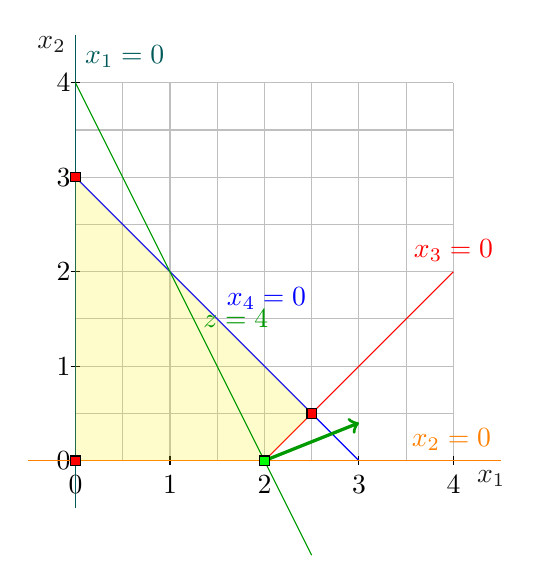
\begin{tikzpicture} [scale=1.2]
\draw[gray!50, thin, step=.5] (0,0) grid (4,4);
\draw[opacity=0.9] (0,0) -- (4.4,0) node[below] {$x_1$};
\draw[opacity=0.9] (0,0) -- (0,4.4) node[left] {$x_2$};

\foreach \x in {0,...,4} \draw (\x,0.05) -- (\x,-0.05) node[below] {\x};
\foreach \y in {0,...,4} \draw (-0.05,\y) -- (0.05,\y) node[left] {\y};

\draw [red](2, 0) --  (4, 2) node[above] {$x_3= 0$};
\draw [blue] (0,3)  -- node[above right] {$x_4=0$} (3,0) ;
\draw [teal!70!black](0,-.5) --  (0,4.5) node[below right] {$x_1=0$}; 
\draw [orange](-.5,0) --  (4.5,0) node[above left] {$x_2=0$}; 

\fill[yellow,opacity=0.2] (0,0) -- (2,0) -- (2.5,0.5) -- (0,3) -- cycle;

\draw [green!60!black] (0, 4)   -- node[right] {$z=4$}  (2.5, -1)  ; % o.f.
\draw [green!60!black, very thick,->](2,0) -- (2+1, 0+2/5); % gradient

\filldraw[fill=red] (-0.05,-0.05) rectangle (0.05,0.05);
\filldraw[fill=red] (2.45,0.45) rectangle (2.55,0.55);
\filldraw[fill=green] (1.95,-0.05) rectangle (2.05,0.05);
\filldraw[fill=red] (-0.05,2.95) rectangle (0.05,3.05);    
\end{tikzpicture} \end{center} 
\end{minipage}
~\vspace{30mm}

\begin{minipage}[t][][b]{.50\linewidth} \vspace{2mm}
\begin{center} \begin{tabular} {l|c||c|c|c|c|c|}  \cline{2-7}
max 	& $z$	& $x_1$ & $x_2$  & $x_3$	& $x_4$	& $rhs$ \\ \cline{2-7}
$z$	    & 1		& 0     & 0     &	 1/2 	&	3/2	&   11/2    \\ \cline{2-7}
$x_1$	& 0		& 1     & 0     &	 1/2 	&	 1/2 &	5/2    \\
$x_2$	& 0		& 0     & 1     &	-1/2 	&	 1/2&	1/2  \\ \cline{2-7}
\end{tabular} \end{center}
\end{minipage}%
\begin{minipage}[t][][b]{.50\linewidth}
\begin{center}  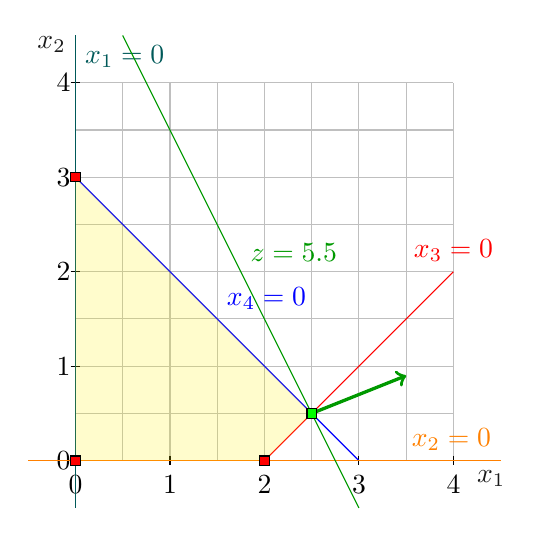
\begin{tikzpicture} [scale=1.2]
\draw[gray!50, thin, step=.5] (0,0) grid (4,4);
\draw[opacity=0.9] (0,0) -- (4.4,0) node[below] {$x_1$};
\draw[opacity=0.9] (0,0) -- (0,4.4) node[left] {$x_2$};

\foreach \x in {0,...,4} \draw (\x,0.05) -- (\x,-0.05) node[below] {\x};
\foreach \y in {0,...,4} \draw (-0.05,\y) -- (0.05,\y) node[left] {\y};

\draw [red](2, 0) --  (4, 2) node[above] {$x_3= 0$};
\draw [blue] (0,3)  -- node[above right] {$x_4=0$} (3,0) ;
\draw [teal!70!black](0,-.5) --  (0,4.5) node[below right] {$x_1=0$}; 
\draw [orange](-.5,0) --  (4.5,0) node[above left] {$x_2=0$}; 

\fill[yellow,opacity=0.2] (0,0) -- (2,0) -- (2.5,0.5) -- (0,3) -- cycle;

\draw [green!60!black] (0.5, 4.5)   -- node[above right] {$z=5.5$}  (3, -0.5)  ; % o.f.
\draw [green!60!black, very thick,->](2.5,0.5) -- (2.5+1, 0.5+2/5); % gradient

\filldraw[fill=red] (-0.05,-0.05) rectangle (0.05,0.05);
\filldraw[fill=green] (2.45,0.45) rectangle (2.55,0.55);
\filldraw[fill=red] (1.95,-0.05) rectangle (2.05,0.05);
\filldraw[fill=red] (-0.05,2.95) rectangle (0.05,3.05);    
\end{tikzpicture} \end{center} 
\end{minipage}

\vspace{10mm} Let's consider this algorithm, and what we know, and see if there are any missing parts, or other information we would find valuable.

\begin{itemize}
\item Unique optimal solution 
\item Multiple optimal solutions
\item Unbounded optimal objective value
\item Empty feasible region (an infeasible LP)
\end{itemize}

\vspace{10mm}{\bf Tableau Formulas:} \\

We can modify the tableau for a particular basis $\mathbf{B}$ using the following formulas:
\begin{center} \begin{tabular} {l|c|c|c|} \cline{2-4}
                    & $z$	        & $x_i$	                       &  $rhs$  \\ \cline{2-4}
 ($z$)         & 1	            & $\mathbf{c_BB^{-1}a_i -c_i}$ & $\mathbf{c_BB^{-1}b}$	    \\
 ($x_B$)  & $\mathbf{0}$	& $\mathbf{B^{-1}a_i}$	       & $\mathbf{B^{-1}b}$  \\ \cline{2-4}
\end{tabular} \end{center}
If we partition the variables, the formulas simplify as follows:
\begin{center} \begin{tabular} {l|c|c|c|c|} \cline{2-5}
       & $z$          & $x_{B}$	 & $x_{N}$                            & $rhs$ \\ \cline{2-5}
$z$    & 1	          & $\mathbf{c_BB^{-1}B-c_B=0}$ & $\mathbf{c_BB^{-1}N-c_{N}}$ & $\mathbf{c_BB^{-1}b}$ \\
$x_B$  & $\mathbf{0}$ & $\mathbf{B^{-1}B=I}$ & $\mathbf{B^{-1}N}$	       & $\mathbf{B^{-1}b}$ \\ \cline{2-5}
\end{tabular} \end{center} 

\bigskip The formulas for the coefficients for rows 1-$m$, that is $\mathbf{B^{-1}a_i}$ (or $\mathbf{B^{-1}A}$ for all the columns on the left-hand side) is fairly straight forward; Multiplying by $\mathbf{B^{-1}}$ is essentially the same as doing the elementary row operations required to get an identity matrix in the basic variable columns.  \\

Now consider the formula $\mathbf{c_BB^{-1}a_i -c_i}$ for the row~0 coefficients. Where did this come from? \\


Consider an expanded basis matrix $\mathbf{\hat{B}}$, which includes the $z$-variable column and row, as follows: $\left[ \begin{array}{cc}
    1 & -\mathbf{c_B} \\
    0 & \mathbf{B} \\
\end{array} \right],$
which yields $\mathbf{\hat{B}^{-1}}$ of $\left[ \begin{array}{cc}
    1 & \mathbf{c_BB^{-1}} \\
    0 & \mathbf{B^{-1}} \\
\end{array} \right],$
and the column for $x_i$ is $[-c_i, \mathbf{a_i}]^T$.  Multiplying these yields $\left[
\begin{array}{cc}
 1         & \mathbf{c_BB^{-1}} \\
\mathbf{0} & \mathbf{B^{-1}} \\
\end{array} \right] \left[
\begin{array}{c}
     -c_i \\
     \mathbf{a_i} \\
\end{array} \right],$
which results in dot product of  $[1,\mathbf{c_BB^{-1}}][-c_i, \mathbf{a_i}] = \mathbf{c_BB^{-1}a_i} - c_i$ for the first element of the resulting column vector. \\

\vspace{5mm} For example, consider the following LP:
\begin{align*}
\mbox{Max~~} & z = 2x_1 + 3x_2  \\
\mbox{s.t.~~}  & 1x_1 + 1x_2 \ge 2 \\
&      4x_1 + 6x_2 \le 9 \\
&      x_1, x_2 \ge 0. 
\end{align*}

For this problem, if we have $x_1$ ad $x_2$ as the basic variables, then \\

$\mathbf{\hat{B}} = \left[ \begin{array}{ccc}
    1 & -2 & -3 \\
    0 &  1 &  1 \\
    0 &  4 &  6 \\
\end{array} \right]$
and $\mathbf{\hat{B}^{-1}} = \left[ \begin{array}{ccc}
    1 &  0  & 1/2   \\
    0 &  3  &  -1/2 \\
    0 &  -2 &  1/2 \\
\end{array} \right],$ \\

and the column for $x_1$ is $[-2, 1, 4]^T$.  \\

When we multiply $\mathbf{\hat{B}^{-1}}$ and $[-2, 1, 4]^T$ we get \\

$\left[\begin{array}{ccccccc}
    1 & 0  & 1/2    &~& -2  & & 0 \\
    0 & 3  & -1/2   &~& 1   &=& 1 \\
    0 & -2 &  1/2   &~& 4   & & 0 \\
\end{array} \right]$


\vspace{10mm}The simplex algorithm again:
\begin{enumerate}
\item Put the LP into a standard form tableau, find a feasible basis $\mathbf{B}$ and  modify the tableau using  $\mathbf{B^{-1}}$ and the tableau formulas.
\item Check optimality, if $\mathbf{c_BB^{-1}a_i -c_i} \ge (\le)~0$ for $i: x_i \in \mathbf{x_N}$ for a maximization (minimization) problem, then the current basic solution is optimal. Stop.
\item Select an entering nonbasic variable using Dantzig's rule, specifically, entering variable $x_i$, where $i =$ \\
$ \text{min (max)}_i~\{ \mathbf{c_BB^{-1}a_i -c_i} < (>)~ 0: (i: x_i \in \mathbf{x_N})\}$ for a maximization (minimization) problem.
\item Select a variable to leave the basis using the ratio test. For entering variable $x_i$ the leaving variable is the basic variable corresponding to row~$j$, where :\\
$\text{min}_j \{[\mathbf{B^{-1}b}]_j/[\mathbf{B}^{-1}\mathbf{a_i}]_j,~( j:j = 1, \cdots,m,~[\mathbf{B}^{-1}\mathbf{a_i}]_j > 0)\}$.
\item Put the  tableau into the proper form for the new basis and go to Step~2.
\end{enumerate}



\underline{\bf Finding an Initial BFS}
When a basic feasible solution is not apparent, we an produce one using {\it artificial variables}.  This {\it artificial} basis is undesirable from the perspective of the original problem, we do not want the artificial variables in our solution, so we penalize them in the objective function, and allow the simplex algorithm to drive them to zero (if possible) and out of the basis.  There are two such methods, the {\bf Big M method} and the {\bf Two-phase method}, which we illustrate below:

\vspace{10mm}  Solve the following LP using the Big M Method and the simplex algorithm:

\begin{align*}
max~~ & z = 9x_1 + 6x_2 \\
s.t.~~
&  3x_1 + 3x_2 \le 9 \\
&  2x_1 - 2x_2 \ge 3 \\
&  2x_1 + 2x_2 \ge 4 \\
& x_1, x_2 \ge 0. \\
\end{align*}

Here is the LP is transformed into standard form by using slack variables $x_3$, $x_4$, and $x_5$, with the required artificial variables $x_6$ and $x_7$, which allow us to easily find an initial basic feasible solution (to the artificial problem).
\begin{eqnarray}
& max  & z_a = 9x_1 + 6x_2 -M x_6 - M x_7 \nonumber \\
& s.t. & 3x_1 + 3x_2 + x_3 = 9 \nonumber \\
&      & 2x_1 - 2x_2 - x_4 + x_6 = 3 \nonumber \\
&      & 2x_1 + 2x_2 - x_5 + x_7 = 4 \nonumber \\
&      & x_i \ge 0,~~ i =1,\cdots,7. \nonumber
\end{eqnarray}

\begin{center} \begin{tabular} {|c|c|c|c|c|c|c|c||c| r} \cline{1-9}
$z$	& $x_1$	& $x_2$	& $x_3$	& $x_4$	& $x_5$	& $x_6$	& $x_7$	& RHS &	ratio \\ \cline{1-9}
1	&	 -9 &	 -6 &	 0 &	  0 &	  0 &	  M &	  M &	0 & \\
0	&	  3 &	  3 &	 1 &	  0 &	  0 &	  0 &	  0 &	9 &	 \\
0	&	  2 &	 -2 &	 0 &	 -1 &	  0 &	  1 &	  0 &	3 & \\
0	&	  2 &	  2 &	 0 &	  0 &	 -1 &	  0 &	  1 &	4 &	 \\
\cline{1-9}
\end{tabular} \end{center}
\noindent This tableau is not in the correct form, it does not represent a basis, the columns for the artificial variables need to be adjusted.

\begin{center} \begin{tabular} {|c|c|c|c|c|c|c|c||c| r} \cline{1-9}
$z$	& $x_1$	  & $x_2$  & $x_3$	& $x_4$	& $x_5$	& $x_6$	& $x_7$	& RHS &	ratio \\ \cline{1-9}
1	& -9 - 4M & -6     &	 0 &	  M &	  M &	  0 &	  0 & -7M &	      \\
0	&	  3   &	     3 &	 1 &	  0 &	  0 &	  0 &	  0 &	9 &	3     \\
0	&	  2   &	    -2 &	 0 &	 -1 &	  0 &	  1 &	  0 &	3 &	3/2   \\
0	&	  2   &	     2 &	 0 &	  0 &	 -1 &	  0 &	  1 &	4 &	2     \\
\cline{1-9}
\end{tabular} \end{center}
\noindent The current solution is not optimal, so $x_1$ enters the basis, and by the ratio test, $x_6$ (an artificial variable) leaves the basis.

\begin{center} \begin{tabular} {|c|c|c|c|c|c|c|c||c| r} \cline{1-9}
$z$	&   $x_1$ & $x_2$   & $x_3$	& $x_4$	& $x_5$	& $x_6$	   & $x_7$	& RHS      & ratio \\
\cline{1-9}
1	&     0   & -15 -4M &	 0 & -9/2 -M &	  M & 9/2 + 2M &	  0 &  27/2 -M &    	\\
0	&	  0   &	     6  &	 1 &	 3/2 &	  0 &	    -3/2 &	  0 &	3/2    & 3/4     \\
0	&	  1   &	    -1  &	 0 &	-1/2 &	  0 &	   1/2 &	  0 &	3/2    & -  	\\
0	&	  0   &	     4  &	 0 &	   1 &	 -1 &	     -1 &	  1 &	  1    & 1/4        	\\ \cline{1-9}
\end{tabular} \end{center}
\noindent The current solution is not optimal, so $x_2$ enters the basis, and by the ratio test, $x_7$ (an artificial variable) leaves the basis.

\begin{center} \begin{tabular} {|c|c|c|c|c|c|c|c||c|r} \cline{1-9}
$z$	&   $x_1$ & $x_2$ & $x_3$ & $x_4$	& $x_5$	& $x_6$	   & $x_7$	& RHS     &	ratio \\
\cline{1-9}
1	&     0   &     0 &	 0    & -3/4    & -15/4 &        - &	  - &  17 1/4 &	   \\
0	&	  0   &	    0 &	 1    &	   0    &	3/2 &	     0 &   -3/2 &	  3   &	-  \\
0	&	  1   &	    0 &	 0    &	-1/4    &  -1/4 &	   1/2 &	1/4 &	  7/4 &	-  	\\
0	&	  0   &	    1 &	 0    &	 1/4    &  -1/4 &	  -1/4 &	1/4 &	  1/4 & 1   \\
\cline{1-9}
\end{tabular} \end{center}
\noindent The current solution is not optimal, so $x_4$ enters the basis, and by the ratio test, $x_2$ leaves the basis.

\begin{center} \begin{tabular} {|c|c|c|c|c|c|c|c||c|r} \cline{1-9}
$z$	&   $x_1$ & $x_2$ & $x_3$ & $x_4$ & $x_5$ & $x_6$ & $x_7$ & RHS     &	ratio \\
\cline{1-9}
1	&     0   &    3  &	 0    & 0     & -9/2  &     - &	    - &  18 &	   \\
0	&	  0   &	    0 &	 1    &	   0  &	  3/2 &	    0 &  -3/2 &	  3     &	-  \\
0	&	  1   &	    1 &	 0    &	0     &  -1/2 &	   0  &	  1/2 &	  2   &	-  	\\
0	&	  0   &	    4 &	 0    &	 1    &  -1   &	  -1 &      1 &	  1    & 1   \\ \cline{1-9}
\end{tabular} \end{center}
\noindent The current solution is not optimal, so $x_5$ enters the basis, and by the ratio test, $x_3$ leaves the basis.

\begin{center} \begin{tabular} {|c|c|c|c|c|c|c|c||c|r} \cline{1-9}
$z$	&   $x_1$ & $x_2$ & $x_3$ & $x_4$ & $x_5$ & $x_6$ & $x_7$ & RHS     &	ratio \\
\cline{1-9}
1	&     0   &    3  &	 3    & 0     & 0  &     - &	    - &  27 &	   \\
0	&	  0   &	    0 &	 2/3  &	  0   &	  1 &	    0 &  -1 &	  2     &	 \\
0	&	  1   &	    1 &	 1/3   &   0  &  0 &	   0  &	  0 &	  3   &  	\\
0	&	  0   &	    4 &	 2/3   &	1 &  0   &	  -1 &     0&	 3    &    \\
\cline{1-9}
\end{tabular} \end{center}
The current solution is optimal! \\

\bigskip Solve the following LP using the Two-phase Method and Simplex Algorithm.
\begin{align*}
max~~ & z = 2x_1 + 3x_2   \\
s.t.~~ 
& 3x_1 + 3x_2 \ge 6  \\
& 2x_1 - 2x_2 \le 2  \\
& -3x_1 + 3x_2 \le 6   \\
& x_1, x_2 \ge 0. 
\end{align*}


%\begin{center} \includegraphics[scale=0.7]{Figs_N/TwoPhase}\end{center}

Here is first phase LP (in standard form), where $x_3$, $x_4$, and $x_5$ are slack variables, and $x_6$ is an artificial variable.
\begin{eqnarray}
& min  & z_a = x_6 \nonumber \\
& s.t. & 3x_1 + 3x_2 - x_3 +x_6 = 6 \nonumber \\
&      & 2x_1 - 2x_2 + x_4 = 2 \nonumber \\
&      & -3x_1 + 3x_2 + x_5 = 6 \nonumber \\
&      & x_i \ge 0,~~ i =1,\cdots,6. \nonumber
\end{eqnarray}
Next, we put the LP into a tableau, which, still is not in the right form for our basic variables ($x_6$, $x_4$, and $x_5$).
\begin{center} \begin{tabular} {|c|c|c|c|c|c|c||c| r} \cline{1-8}
$z$	& $x_1$	& $x_2$	& $x_3$	& $x_4$	& $x_5$	& $x_6$	&  RHS & ratio \\ \cline{1-8}
1	&	  0 &	  0 &	 0 &	  0 &	  0 &	 -1 &    0 & \\
0	&	  3 &	  3 &	-1 &	  0 &	  0 &	  1 &	 6 & \\
0	&	  2 &	 -2 &	 0 &	  1 &	  0 &	  0 &	 2 & \\
0	&	  -3 &	  3 &	 0 &	  0 &	  1 &	  0 &	 6 & \\ \cline{1-8}
\end{tabular} \end{center}
To remedy this, we use row operation to modify the row 0 coefficients, yielding the following:
\begin{center} \begin{tabular} {|c|c|c|c|c|c|c||c| r} \cline{1-8}
$z$	& $x_1$	& $x_2$	& $x_3$	& $x_4$	& $x_5$	& $x_6$	&  RHS & ratio \\ \cline{1-8}
1	&	  3 &	  3 &	 -1 &	  0 &	  0 &	  0 &    6 &   \\
0	&	  3 &	  3 &	-1 &	  0 &	  0 &	  1 &	 6 &  2 \\
0	&	  2 &	 -2 &	 0 &	  1 &	  0 &	  0 &	 2 &  - \\
0	&	  -3 &	  3 &	 0 &	  0 &	  1 &	  0 &	 6 &  2 \\ \cline{1-8}
\end{tabular} \end{center}
The current solution is not optimal, either $x_1$ or $x_2$ can enter the basis, let's choose $x_2$. Then by the ratio test, either $x_6$ (an artificial variable) or $x_5$ (a slack variable) can leaves the basis.  Let's choose $x_6$.
\begin{center} \begin{tabular} {|c|c|c|c|c|c|c||c| r} \cline{1-8}
$z$	& $x_1$	& $x_2$	& $x_3$	& $x_4$	& $x_5$	& $x_6$	&  RHS & ratio \\ \cline{1-8}
1	&	  0 &	  0 &	 0 &	  0 &	  0 &  -1 &    0 & \\
0	&	  1 &	  1 &	-1/3 &	  0 &	  0 &   1/3 &	 2 & \\
0	&	  4 &	  0 &	-2/3 &	  1 &	  0 &   2/3 &	 6 & \\
0	&	 -6 &	  0 &	 1 &	  0 &	  1 &	 -1 &	 0 & \\ \cline{1-8}
\end{tabular} \end{center}
The current solution is optimal, so we end the first phase with a basic feasible solution to the original problem, with $x_2$, $x_4$, and $x_5$ as the basic variables.  Now we provide a new row zero that corresponds to the original problem.

\begin{center} \begin{tabular} {|c|c|c|c|c|c|c||c| r} \cline{1-8}
$z$	& $x_1$	& $x_2$	& $x_3$	& $x_4$	& $x_5$	& $x_6$	&  RHS & ratio \\ \cline{1-8}
1	&	  1 &	  0 &	 -1 &	  0 &	  0 &	  0 &   6 & \\
0	&	  1 &	  1 &	-1/3 &	  0 &	  0 &	  1/3 &	 2 &   \\
0	&	  4 &	  0 &	-2/3 &	  1 &	  0 &	  2/3 &	 6 &  \\
0	&	 -6 &	  0 &	 1 &	  0 &	  1 &	  -1 &	 0 &  \\ \cline{1-8}
\end{tabular} \end{center}

\begin{center} \begin{tabular} {|c|c|c|c|c|c|c||c| r} \cline{1-8}
$z$	& $x_1$	& $x_2$	& $x_3$	& $x_4$	& $x_5$	& $x_6$	&  RHS & ratio \\ \cline{1-8}
1	&	 -5 &	  0 &	  0 &	  0 &	  1 &	  -1 &   6 & \\
0	&	 -1 &	  1 &	  0 &	  0 &	1/3 &	  0 &	 2 &   \\
0	&	  0 &	  0 &	  0 &	  1 &	2/3 &	  0 &	 6 &  \\
0	&	 -6 &	  0 &	  1 &	  0 &	  1 &	  -1 &	 0 &  \\ \cline{1-8}
\end{tabular} \end{center}
From this tableau we can see that the LP is unbounded and an extreme point is [0, 2, 0, 6,0] and an extreme direction is [1, 1, 6, 0, 0].




\underline{\bf Degeneracy and the Simplex Algorithm}
\begin{comment}
$\mathbf {n} \cdot (\mathbf {r} -\mathbf {r} _{0})=0.$
(The dot here means a dot (scalar) product.) Expanded this becomes

$a(x-x_{0})+b(y-y_{0})+c(z-z_{0})=0$
which is the point-normal form of the equation of a plane.  This is just a linear equation

$ax+by+cz+d=0$,
where

$d=-(ax_{0}+by_{0}+cz_{0}).$  
Conversely, it is easily shown that if a, b, c and d are constants and a, b, and c are not all zero, then the graph of the equation

$ax+by+cz+d=0$ is a plane having the vector 

$\mathbf{ n} = (a, b, c)$ as a normal. 

This plane can also be described by the "point and a normal vector" prescription above. A suitable normal vector is given by the cross product
${\mathbf {n}}=({\mathbf {p}}_{2}-{\mathbf {p}}_{1})\times ({\mathbf {p}}_{3}-{\mathbf {p}}_{1})$,

and the point r0 can be taken to be any of the given points p1,p2 or p3[6] (or any other point in the plane).
Let p1=(x1, y1, z1), p2=(x2, y2, z2), and p3=(x3, y3, z3) be non-collinear points.

${\displaystyle \mathbf {w\times v} ={\begin{vmatrix}\mathbf {i} &\mathbf {j} &\mathbf {k} \\w_{1}&w_{2}&w_{3}\\v_{1}&v_{2}&v_{3}\\\end{vmatrix}}}$

${\displaystyle {\begin{aligned}\mathbf {w\times v} &={\begin{vmatrix}w_{2}&w_{3}\\v_{2}&v_{3}\end{vmatrix}}\mathbf {i} -{\begin{vmatrix}w_{1}&w_{3}\\v_{1}&v_{3}\end{vmatrix}}\mathbf {j} +{\begin{vmatrix}w_{1}&w_{2}\\v_{1}&v_{2}\end{vmatrix}}\mathbf {k} \\&=(w_{2}v_{3}-w_{3}v_{2})\mathbf {i} +(w_{3}v_{1}-w_{1}v_{3})\mathbf {j} +(w_{1}v_{2}-w_{2}v_{1})\mathbf {k} ,\end{aligned}}}$
\end{comment}

Degeneracy must be considered in the simplex algorithm, as it causes some trouble.  For instance, it might mislead us into thinking there are multiple optimal solutions, or provide faulty insight.  Further, the algorithm as described can {\it cycle}, that is, remain on a degenerate extreme point repeatedly cycling through a subset of bases that represent that point, never leaving. 

\begin{center} \begin{tabular} {c|c|c|c|c|c|c|c|c|c|} \cline{2-10}
min &$z$	& $x_1$ & $x_2$ & $x_3$	& $x_4$	&  $x_5 $& $x_6$ & $x_7$ & $rhs$ \\ \cline{2-10}
       &1		& 0 		  & 0         &	 0 	    &	  3/4     &   -20 & 1/2 & -6  &     0    \\ \cline{2-10}
       &0		&	 1       &	    0   &	 0 			&	  1/4 		&	-8 & -1 &   9 &   0	  \\
       &0		&	 0     &	    1      &	 0 		&	  1 /2		&	 -12 & -1/2 & 3 & 0   \\ 
       &0		&	 0     &	    0      &	 1 		&	  0		&	 0 & 1 & 0 &1   \\ \cline{2-10}
\end{tabular} \end{center}


\bigskip  Solve the following LP using the Simplex Algorithm:
\begin{eqnarray}
& \max  & z = 40x_1 + 30x_2 \nonumber \\
& s.t. & 6x_1 + 4x_2 \le 40 \nonumber \\
&      & 4x_1 + 2x_2 \le 20 \nonumber \\
&      & x_1, x_2 \ge 0. \nonumber
\end{eqnarray}

By adding slack variables, we have the following tableau.
\begin{table}[h!] \begin{center} \begin{tabular} {|c|c|c|c|c||c|}
\hline
$z$ & $x_1$ & $x_2$ & $s_1$ & $s_2$ & RHS \\ \hline
  1 & -40 & -30 & 0   & 0   & 0  \\
  0 &   6 &   4 & 1   & 0   & 40 \\
  0 &   4 &   2 & 0   & 1   & 20 \\ \hline
\end{tabular} \end{center} \end{table}
Luckily, this tableau represents a basis, where BV=$\{s_1, s_2\}$, but by inspecting the row 0 (objective function row) coefficients, we can see that this is not optimal. By Dantzig's Rule, we enter $x_1$ into the basis, and by the ratio test we see that $s_2$ leaves the basis.  By performing elementary row operations, we obtain the following tableau for
the new basis BV=$\{s_1, x_1\}$.
\begin{center} \begin{tabular} {|c|c|c|c|c||c|} \hline
$z$ & $x_1$ & $x_2$ & $s_1$ & $s_2$ & RHS \\
\hline
  1 &     0 &   -10 & 0     &    10 & 200 \\
  0 &     0 &     1 & 1     &  -3/2 & 10 \\
  0 &     1 &   1/2 & 0     &   1/4 &  5 \\
\hline
\end{tabular} \end{center}

This tableau is not optimal, entering $x_2$ into the basis can improve the objective function value. The basic variables $s_1$ and $x_1$ tie in the ration test.  If we have $x_1$ leave the basis, we get the following tableau (BV=$\{s_1, x_2\}$).
\begin{center} \begin{tabular} {|c|c|c|c|c||c|}
\hline
$z$ & $x_1$ & $x_2$ & $s_1$ & $s_2$ & RHS \\
\hline
  1 &    20 &     0 &     0 &    15 & 300 \\
  0 &    -2 &     0 &     1 &    -2 &  0 \\
  0 &     2 &     1 &     0 &   1/2 &  10 \\ \hline
\end{tabular} \end{center}
This is an optimal tableau, with an objective function value of 300,  If instead of $x_1$ leaving the basis, suppose $s_1$ left, this would lead to the following tableau (BV=$\{x_2, x_1\}$).
\begin{center} \begin{tabular} {|c|c|c|c|c||c|} \hline
$z$ & $x_1$ & $x_2$ & $s_1$ & $s_2$ & RHS \\
\hline
  1 &     0 &     0 &    10 &    -5 & 300 \\
  0 &     0 &     1 &     1 &  -3/2 &  10 \\
  0 &     1 &     0 &  -1/2 &     1 &   0 \\ \hline
\end{tabular} \end{center}
This tableau does not look optimal, yet the objective function value is the same as the optimal solution's. This occurs because the optimal extreme point is a degenerate.% as the following figure shows.


%\begin{center} \includegraphics[scale=0.7]{Figs_N/degen} \end{center}

\subsubsection{Dual Simplex Algorithm}
The dual simplex algorithm is essentially performing the simplex algorithm, on the dual problem, on the primal tableau. Remember, the Simplex algorithm, in relation to the KKT conditions, maintains primal feasibility, complementary slackness, and strives for dual feasibility. The dual simplex algorithm maintains dual feasibility, complementary slackness, and strives for primal feasibility. \\

\begin{enumerate}
\item Pick the row with the smallest $\bar{b}_i$, where $\bar{b}_i < 0$ ($\mathbf{\bar{b}} = \mathbf{B^{-1}b}$), this corresponds to the leaving variable.
\item Pick a column with the minimum $\{|z_j -c_j/y_{ij}|:y_{ij} < 0\}$, this corresponds to the entering variable.
\item Pivot, and repeat until primal feasibility is achieved.
\end{enumerate}



\subsubsection{Primal-Dual Algorithm}
The primal dual algorithm is another method for solving LPs. This algorithm starts with a feasible dual solution (not necessarily basic) and searches for a primal feasible solution will maintaining complementary slackness between the primal and dual solutions.  Consider the following primal dual pair:

\begin{align*}
&(P):\min\{\mathbf{cx}: \mathbf{Ax} = \mathbf{b}, \mathbf{x} \ge 0\} \\
&(D):\max\{{\bf wb}: \mathbf{wA} \le \mathbf{c}, {\bf w}~urs\}.
\end{align*}
To solve $P$ using the primal-dual algorithm, first find a feasible solution to $D$, it does not necessarily have to be basic, and form the following restricted primal problem:
$$(P_R):\min\{z_R= {\bf 1x^a}: \mathbf{a_j}x_j+\mathbf{x^a\mathbf} = \mathbf{b}, x_j \ge 0,~ j \in Q,~\mathbf{x^a} \ge \mathbf{0}\},$$
where $Q=\{j:wa_j = c_j\}$, that is, $Q$ is the set of indexes for binding dual constraints, and $x_j, j \in Q$ are the primal variables that can be non-zero given the current dual solution and complementary slackness. The vector $\mathbf{x^a}$ is a vector of artificial variables; this problem looks very similar to the phase~1 problem in the two-phase method.  The objective is the same, to find a basic feasible primal solution, but here we use a {\it restricted} or limited number of primal variables, those with indexes in set $Q$.\\

Solve $P_R$ (using simplex) and if $z_R=0$, stop, the solution is optimal for $P$ because we have satisfied the KKT conditions, else let $\mathbf(v)^*$ be the corresponding optimal dual solution $D_R$.

$$D_R:\max\{\mathbf{vb}: \mathbf{va_j }\le 0,~ i \in Q, \mathbf{v} \le 1, \mathbf{v}~ urs\}.$$

Note that for each $j \in Q$, $\mathbf{v^*a_j} \le 0$. For $i \notin Q$ calculate $\mathbf{v^*a_i}$, if $\mathbf{v^*a_i} > 0$ then $x_i$ can be added to the restricted primal to improve $z_R$.  To get $x_i$ into $Q$ we must modify the original dual solution $\mathbf{w}$, first we calculate $\theta$.

$$ \theta = \min_{i \notin Q} \{|(\mathbf{wa_i}-c_i)|/\mathbf{v^*a_i} : \mathbf{v^*a_i} > 0\}  > 0$$ 

We take the absolute value of $\mathbf{wa_i}-c_i)$ because if the primal problem is a minimization, this term will always be non-positive, for a primal maximization this will always be non-negative (thus the absolute value is not needed). \\

We then replace $\mathbf{w}$ by $\mathbf{w}+\theta\mathbf{v^*}$.  We use this $\theta$-step like a ratio test, changing the current dual solution such that we can enter a new primal variable into the restricted primal, one that will improve the solution (and move us closer to feasibility), while maintaining dual feasibility and complementary slackness.  \\

If we think about this algorithm on a tableau, we get the following formulas, where the $z_P$ row corresponds to our dual solution, and defines the set $Q$, and simplex is performed on on the restricted problem (using row $z^R_P$ for the objective function row, and using column defined by $Q$). 

\begin{center} \begin{tabular} {c|c|c|c|c|c|} \cline{2-6}       
		& $z$ 	& $\mathbf{x}$ 			& $\mathbf{x^s}$ 		& $\mathbf{x^a}$	& rhs  \\ \cline{2-6}\cline{2-6} 
$z_P$  	& 1  	& $\mathbf{wa_i}-c_i$	& $\mathbf{wa_i}$		& 0					& 0    \\ \cline{2-6}
$z^R_P$ & 1		& $\mathbf{va_i} $   	& $\mathbf{va_i} $		& $\mathbf{va_i}-1$ & 0    \\ \cline{2-6} \cline{2-6}       
		& 0     & $\mathbf{B^{-1}a_i}$	& $\mathbf{B^{-1}a_i}$& $\mathbf{B^{-1}a_i}$ 	& $\mathbf{B^{-1}b}$   \\ \cline{2-6}
\end{tabular} \end{center}


\begin{example}{Primal-dual algorithm}{primal-dual-alg}
Consider again the following LP and solve using the primal-dual algorithm, using a starting feasible dual solution of $\mathbf{w} = [10,0,0]$.
\end{example}
\begin{solution}

\begin{eqnarray}
& \max  & 18x_1 + 16x_2 + 10x_3  \nonumber \\
& s.t. & 2x_1 + 2x_2 + 1x_3 +x^s_4 = 21~~ (w_1) \nonumber \\
&      & 3x_1 + 2x_2 + 2x_3 + x^s_5 = 23~~ (w_2) \nonumber \\
&      & 1x_1 + 2x_2 + 1x_3 +x_6 = 17~~ (w_3) \nonumber \\
&      & x_1, x_2, x_3, x_4, x_5, x_6 \ge 0. \nonumber
\end{eqnarray}
\begin{eqnarray}
D1:& \min  & 21w_1 +23w_2 +17w_3  \nonumber \\
   & s.t. & 2w_1 +3w_2 + 1w_3 \ge 18~~ (x_1) \nonumber \\
   &      & 2w_1 +2w_2 + 2w_3 \ge 16~~ (x_2) \nonumber \\
   &      & 1w_1 +2w_2 + 1w_3 \ge 10~~ (x_3) \nonumber \\
   &      & w_1, w_2, w_3 \ge 0. \nonumber
\end{eqnarray}
Use the modified tableau method, and write $Q$ and the restricted problem for each step.  Be able to explain the complete process.

For $\mathbf{w} = [10,0,0]$ we have $Q=\{3,5,6\}$
\begin{center} \begin{tabular} {|c|c|c|c|c|c|c|c|c|}
\hline       & $x_1$ & $x_2$ & $x_3$ & $x^s_4$ & $x^s_5$ & $x^s_6$ &$x^a_7$ & rhs   \\ \hline
\hline $z$   & 2     & 4     & 0      & 10   & 0     & 0     &  0    & 210   \\
\hline $z_R$ & 0     & 0     & 0      & 0    & 0     & 0     & -1    & 0     \\
\hline       & 2     & 2     & 1      & 1    & 0     & 0     & 1     & 21    \\
\hline       & 3     & 2     & 2      & 0    & 1     & 0     & 0     & 23   \\
\hline       & 1     & 2     & 1      & 0    & 0     & 1     & 0     & 17   \\ \hline
\end{tabular} \end{center} \label{T1}

We need to make a minor adjustment to the artificial variable column.
\begin{center} \begin{tabular} {|c|c|c|c|c|c|c|c|c|c|} \hline       
			& $z_P$ & $x_1$ & $x_2$ & $x_3$ & $x^s_4$ 	& $x^s_5$ 	& $x^s_6$ 	& $x^a_7$ 	& rhs  \\ \hline\hline 
$z_P$ 	&  1  	& 2    	& 4     & 0     & 10   		& 0     	& 0  & 0   & 210   \\ \hline 
$z_R$ 	&  1	& 2    	& 2     & \hi 1     & 1    		& \hi 0     	&\hi 0     	&\hi 0     	&\hi 21    \\ \hline \hline       
			&  0    & 2     & 2     & \hi 1     & 1    		& \hi 0     	& \hi 0     	&\hi 1 &\hi  21    \\ \hline       
		& 0 	& 3     & 2     & \hi 2     & 0    		& \hi 1     	&\hi 0     	&\hi 0     	&\hi 23   \\ \hline       
		& 0 	& 1     & 2     & \hi 1      & 0    	&\hi  0     	&\hi 1     	&\hi 0     	&\hi 17   \\ \hline
\end{tabular} \end{center}

$x_3$ enters the restricted basis and $x^s_5$ leaves the restricted basis, resulting in the following tableau:
\begin{center} \begin{tabular} {|c|c|c|c|c|c|c|c|c|} \hline      
         & $x_1$ & $x_2$ & $x_3$  & $x^s_4$ 	& $x^s_5$ 	& $x^s_6$ & $x^a_7$ & rhs  \\ \hline \hline 
$z$   & 2     & 4     & 0      & 10   & 0     & 0     & 0     & 210   \\ \hline 
$z_R$ & 1/2   & 1     &\hi 0      & 1     &\hi -1/2  &\hi 0     &\hi 0      &\hi 19/2   \\ \hline \hline
       & 1/2   & 1     &\hi 0      & 1     &\hi -1/2  &\hi0     &\hi 1      &\hi 19/2   \\ \hline 
      & 3/2   & 1     &\hi 1      & 0     &\hi 1/2   &\hi 0     &\hi 0      &\hi 23/2   \\ \hline 
      & -1/2  & 1     &\hi 0      & 0     &\hi -1/2  &\hi 1     &\hi 0      &\hi 11/2   \\ \hline
\end{tabular} \end{center}

To find $\Theta$ we take the minimum of 4/1 and 2/(1/2), which are equal, and thus $\Theta=4$, using this we adjust the $z$-row, yielding the following tableau. Notice that this operation ensures that the $z$-row remains non-negative. Now $Q=\{1,2,3,6\}$. 

\begin{center} \begin{tabular} {|c|c|c|c|c|c|c|c|c|} \hline      
         & $x_1$ & $x_2$ & $x_3$  & $x^s_4$ 	& $x^s_5$ 	& $x^s_6$ & $x^a_7$ & rhs  \\ \hline \hline 
$z$   & 0     & 0     & 0      & 6   & 2     & 0     & 0     & 172   \\ \hline 
$z_R$ &\hi 1/2   &\hi 1     &\hi 0      & 1     & -1/2  &\hi 0     &\hi 0      &\hi 19/2   \\ \hline \hline
       &\hi 1/2   &\hi 1     &\hi 0      & 1     & -1/2  &\hi0     &\hi 1      &\hi 19/2   \\ \hline 
      &\hi 3/2   &\hi1     &\hi 1      & 0     & 1/2   &\hi 0     &\hi 0      &\hi 23/2   \\ \hline 
      &\hi -1/2  &\hi 1     &\hi 0      & 0     & -1/2  &\hi 1     &\hi 0      &\hi 11/2   \\ \hline
\end{tabular} \end{center}
$x_2$ enters the basis (of the restricted problem) and $x_6$ leaves.
\begin{center} \begin{tabular} {|c|c|c|c|c|c|c|c|c|}
\hline       & $x_1$ & $x_2$ & $x_3$  & $x^s_4$ 	& $x^s_5$ 	& $x^s_6$ & $x^a_7$ & rhs  \\ \hline \hline
$z$    	& 0     & 0     & 0      & 6     & 2     & 0     & 0      & 172 \\ \hline
$z_R$ 	&\hi 1     &\hi 0     &\hi 0      & 1     & 0     &\hi -1    &\hi 0      &\hi 4   \\ \hline \hline
      &\hi 1     &\hi 0     &\hi 0      & 1     & 0     & \hi-1    &\hi 1      &\hi 4   \\ \hline 
      &\hi 2     &\hi 0     &\hi 1      & 0     & 1     &\hi -1    &\hi 0      &\hi 6   \\ \hline 
       &\hi -1/2  &\hi 1     &\hi 0      & 0     & -1/2  &\hi 1     &\hi 0      &\hi 11/2   \\ \hline
\end{tabular} \end{center}

This is not an optimal solution, so now $x_1$ enters the restricted basis and $x_3$ leaves.
\begin{center} \begin{tabular} {|c|c|c|c|c|c|c|c|c|}
\hline       & $x_1$ & $x_2$ & $x_3$  & $x^s_4$ 	& $x^s_5$ 	& $x^s_6$& $x^a_7$ & rhs  \\ \hline
\hline $z$   & 0     & 0     & 0      & 6     & 2     & 0     & 0      & 172 \\
\hline $z_R$ &\hi  0     &\hi  0     &\hi  -1/2   & 1     & -1/2  &\hi  -1/2  &\hi  0      &\hi  1   \\ \hline
\hline       &\hi  0     &\hi  0     &\hi  -1/2   & 1     & -1/2  &\hi  -1/2  &\hi  1      &\hi  1   \\
\hline       &\hi  1     &\hi  0     &\hi  1/2    & 0     & 1/2   &\hi  -1/2  &\hi  0      &\hi  3   \\
\hline       &\hi  0     &\hi  1     &\hi  1/4    & 0     & -1/4  &\hi  3/4   &\hi  0      &\hi  7   \\ \hline
\end{tabular} \end{center}

\medskip \noindent Here $\Theta=6$, which yields the following, having Now $Q=\{1,2,4\}$; we can see that $x_4$ enters and $a_1$ leaves, which will change the $z_R$-row, this makes the restricted primal optimal, but does not change any other rows, and thus this is the optimal solution.
\begin{center} \begin{tabular} {|c|c|c|c|c|c|c|c|c|} \hline       
			& $x_1$ & $x_2$ & $x_3$  & $x^s_4$ 	& $x^s_5$ 	& $x^s_6$& $x^a_7$ & rhs  \\ \hline \hline
$z$   	& 0     & 0     & 3      & 0     & 5     & 3     & 0      & 166 \\ \hline
$z_R$ 	& 0     & 0     &  -1/2   &1     & -1/2  & -1/2  & 0      & 1   \\ \hline \hline
      		& 0     & 0     & -1/2   & 1     & -1/2  & -1/2  & 1      & 1   \\ \hline 
      		& 1     & 0     & 1/2    & 0     & 1/2   & -1/2  & 0      & 3   \\ \hline 
      		& 0     & 1     & 1/4    & 0     & -1/4  & 3/4   & 0      & 7   \\ \hline
\end{tabular} \end{center}
\end{solution}
